\chapter{Native compound types}
\label{chap:compound}

This chapter specifies the native compound types, and lists the casting, unary,
binary and index operations permitted on each. Unlike the scalar types of
Chapter~\ref{chap:scalars}, a compound type usually borrows the values it holds,
so its mutability is a subject in its own right, and is treated here alongside
each type.

The \token{pragma} operations that apply to compound types are not covered here;
they belong to Chapter~\ref{chap:conditional_compilation}.

\minitoc%

\section{Preamble}%
\label{sec:compound:preamble_compound_types}

Before presenting the specifications of the different compound types, let's
define some useful language elements.

\begin{itemize}
\item \textit{Data borrowing} -- A data borrowing value is a value that points
  to data that is not automatically copied when the value is copied. The
  simplest example of data borrowing is the use of a pointer type, where the
  value of the pointer provides information about a memory address containing
  data. The data that the pointer points to is not copied when the pointer is
  copied. An illustration of this is given in Figure~\ref{fig:compound:data_borrowing}.
  In this example, both variables \token{x} and \token{y} borrow the data
  located on the heap at address \token{0xfa45b987}. Copying the value of the
  variable \token{y} to another variable does not make a copy of the borrowed
  value (which is on the heap), but only copies the value directly inside
  \token{y}, which in this case is on the stack. The borrowed data can be on
  the stack or on the heap, and the same can be said for the borrowing data.
  Such memory is called ``borrowed'' because it can live longer than the value
  pointing to it, and the pointer only temporarily borrows its value for reading
  or writing.

  In the case of borrowing data, mutability is crucial because multiple variables
  refer to the same segment of memory. This can lead to unpredictable side
  effects. Memory mutability governs such behaviour, and ensures that
  only a few variables have mutable access to values. Most importantly, it is a
  safeguard against the accidental creation of mutable memory references.


\end{itemize}

\begin{figure}[h]
  \centering
  \begin{adjustbox}{max width=\linewidth}
    \begin{tikzpicture}
      \foreach \name/\y/\base in {x/0/0, y/-1.8/24} {
        \node[memcell] (\name len) at (0, \y) {3};
        \node[memaddr, right=0mm of \name len] (\name ptr) {};
        \node[memcell, right=0mm of \name ptr] (\name blk) {\dots};
        \foreach \field/\off [count=\k from 0] in {len/0, ptr/8, blk/16} {
          \pgfmathtruncatemacro{\at}{\base + \off}
          \node[memnote, above=0.5mm of \name\field] {\field\ +\at};
        }
      }
      \node[cflab, left=3mm of xlen] (xn) {\token{x}};
      \node[cflab, left=3mm of ylen] (yn) {\token{y}};
      \node[memframe, fit=(xn)(xblk)(yn)(yblk), inner ysep=4mm] (foo) {};
      \node[memtitle] at ([xshift=2mm]foo.north west) {foo};

      \foreach \value [count=\i from 0] in {1, 2, 3} {
        \node[memcell] (h\i) at (6.4 + \i * 1.0, -1.4) {\value};
      }
      \node[memnote, above=0.5mm of h0] {0xfa45b987};
      \draw[mempoint] (xptr.center) .. controls +(0, -1.0) and +(-1.5, 0) .. (h0.west);
      \draw[mempoint] (yptr.center) .. controls +(0, -1.0) and +(-1.5, 0) .. (h0.west);

      \node[memregion] (stack) at ($(foo.north) + (0, 5mm)$) {stack};
      \node[memregion] at (h1 |- stack.base) {heap};
      \draw[memsep] (5.2, 1.4) -- (5.2, -3.2);
    \end{tikzpicture}
  \end{adjustbox}
  \caption{\label{fig:compound:data_borrowing} Two slices \token{x} and
    \token{y} of the frame of \token{foo}, borrowing the same data. Each slice
    is 24 bytes on the stack, its offset in the frame above each word. Both
    point to the elements at address \token{0xfa45b987} on the heap, which are
    not part of either value.}
\end{figure}


\begin{itemize}
  \setlength\itemsep{-4pt}
\item \textit{Data movement} -- Data movement is the process of copying a value
  from one segment of memory to another. This can be done by allocation, memory
  copy (or deep copy), function calls and other operations. Data movements are
  always explicit, which ensures that no unwanted copies are made that could
  potentially slow down the program.

\item \textit{lvalue} -- An lvalue refers to the left operand in a \textit{data
  movement} operation. In other words, it is an expression that refers to a
  segment of memory that is modified as a result of the \textit{data movement}.
  An lvalue can take various forms, including a simple variable, a function
  parameter, an index operation, and more.

\item \textit{rvalue} -- An rvalue is the right operand involved in a
  \textit{data movement} operation. An rvalue can be aliased (using the keyword
  \token{alias}), referenced (keyword \token{ref}), copied with
  (\token{copy}, \token{dcopy}), or it can be implicit. These keywords, and the
  levels of mutability the rest of this chapter refers to, are specified in
  Chapter~\ref{chap:memory}, the implicit cases in
  Section~\ref{sec:memory:memory_movement} and mutability itself in
  Section~\ref{sec:memory:variable_mutability}. Implicit means that
  the \textit{data movement} does not borrow mutable data and can therefore be
  allowed implicitly. In the case of an implicit \textit{data movement} there is
  no copying of borrowed data and there is no new borrowing of mutable memory.

\end{itemize}







\section{Pointers}%
\label{sec:compound:pointer_type}

Pointers are values storing an address of memory. Pointer types are described
using the \token{*} token followed by a type (e.g. \token{*i32} describing a
pointer to a \token{i32} value). In the beta version of Ymir (compiler written
in C++) the operator \token{\&} was used, it was changed as it was also used to
refer to object instances that are in a way pointers but have very different
behavior.

\subsection{Literals}

The keyword \token{null} describes a pointer pointing to nowhere.
This is the only literal that can be used as a pointer value.

\subsection{Construction}

To construct a pointer, the unary operator \token{\&} can be used on an lvalue
(for example, a variable). This operator returns the address of the value
referenced by the operand, i.e. \token{\&a} returns the address of the segment
of memory referenced by the variable \token{a}. More simply, the operation
retrieves the address of the variable \token{a}.

\begin{lstlisting}[style=coloredverbatim]
let a = 12;
let b: *i32 = &a;

println(b); // the address of a, in hexadecimal
\end{lstlisting}

\subsection{Mutability and memory alignment}

A pointer value is a machine address, so its size and its alignment are those of
a \token{usize}, that is 8 bytes on a 64-bit system, regardless of the type of
the value it points to.
\smallskip

Because pointers borrow data from another value (value pointed by the pointer),
their mutability is important. A pointer has two levels of mutability:
\begin{enumerate}
  \setlength\itemsep{-4pt}
\item \token{mut *T}, In this case, the pointer can be changed, but the value
  inside the pointer cannot be changed.
\item \token{mut *(mut T)}, In this case, both the value to which the pointer
  is pointing and the pointer itself can be changed.
\end{enumerate}

A mutable pointer (\textit{level 1}) means that if the pointer is contained
inside another compound type or variable, then the value it points to can be
changed. Checking for mutability is done at compile time when borrowing a value
to construct a pointer value.
\smallskip

\begin{lstlisting}[style=coloredverbatimError]
let dmut a: *i32 = null;

let b = 12;
a = &b; // not allowed 'b' is not mutable
*a = 24; // but it would be modified by this operation


let mut c = 11;
a = &c; // allowed c is mutable
*a = 24; // modify the value of c is allowed
\end{lstlisting}

\smallskip
The keyword \token{alias} must be used on the right operand when data borrowing
is transferred to the left operand. In practice, this means that if the
mutability of the left operand is second level (i.e. \token{mut *(mut T)}), the
keyword \token{alias} must be used, and the right operand must also be second
level mutable. The keyword can be omitted if the aliasing is obvious (i.e. by
function return, or construction such as the unary operator \token{\&}).

\subsection{Properties}

Pointer type properties can be accessed using the \token{::} operator on a type
expression. The properties are as follows:

\begin{center}\begin{adjustbox}{max width=\linewidth}
  \begin{tabular}{|l|ll|}
    \hline
    Name & Meaning & Type\\
    \hline
    \hline
    \token{init} & The initial value \token{null} & \token{typeof(x)}\\
    \hline
    \token{typeid} & A string encoding the name of the type & \token{[c8]} \\
    \hline
  \end{tabular}
\end{adjustbox}\end{center}

\subsection{Explicit casting}

There is no implicit conversion between pointer types, even when the pointed-to
types are themselves convertible. A pointer type can however be cast to any
pointer type using the cast operator \token{cast!T(V)}. A pointer is a really low-level type with few guarantees,
but some operations rely on this possibility to perform generic operations
(common trait \token{Packable} for example). The mutability of the result is
the same as the mutability of the operand if the value is explicitly aliased; it is
immutable otherwise. This is the only allowed cast on pointer types.
\smallskip

\begin{lstlisting}[style=coloredverbatimError]
  let dmut a: [i32]  = copy [12];
  let dmut b: *[i32] = &a;

  // c : dmut *[f32];
  let dmut c = cast!{*[f32]}(alias b);

  // not allowed, from *[f32] to dmut *[f32];
  let dmut d = cast!{*[f32]}(b);
\end{lstlisting}

\subsection{Unary operators}

The unary operator \token{*} is used on a pointer value to dereference it and
access the value pointed to by the pointer. This operation is unsafe, can only
be used in an \token{unsafe} context, and may cause the program to crash. If the
operation does not crash, it does not necessarily mean that the pointer was
created correctly.
\smallskip

\begin{lstlisting}[style=coloredverbatim]
let i = 10;
let x = &i;

unsafe {
  let j = *x;
  println(j); // 10
}
\end{lstlisting}

\subsection{Binary operators}

Binary operators are divided into three groups:
\begin{itemize}
  \setlength\itemsep{-4pt}
\item Arithmetic: Pointer arithmetic is allowed with a \token{usize} as the
  right operand. Unlike the C language, the arithmetic does not depend on the
  size of the data pointed to by the pointer. The operation adds a number of
  bytes to the address, which means that the addition operation with a left
  operand whose value is \token{0xabc0} and a right operand \token{8us} will
  always have the value \token{0xabc8}, regardless of the type of content
  pointed to by the pointer. The behaviour is not the same with the index
  operator. The type of the result of the operation is always the same as the
  type of the left operand.

  \begin{center}\begin{adjustbox}{max width=1\linewidth}
    \begin{tabular}{|c|lll|}
      \hline
      Operator & Operation & Commutative & Example \\
      \hline
      \hline
      \token{+} & Addition & Yes & \token{&a + 2us} \\
      \token{-} & Subtraction & No & \token{&a - 2us} \\
      \hline
    \end{tabular}
  \end{adjustbox}\end{center}

\item Comparison: Comparison operators always return a value of type \token{bool}
  and can only be used if the two operands are of the same pointer type (e.g.
  \token{*i32} with \token{*i32}).

  \begin{center}\begin{adjustbox}{max width=1\linewidth}
      \begin{threeparttable}
        \begin{tabular}{|c|lll|}
          \hline
          Operator & Operation & Commutative & Example \\
          \hline
          \hline
          \token{==} & Equality test & Yes & \token{(&a == &a) == true}\\
          \token{!=} & Inequality test & Yes & \token{(&a != &a) == false}\\
          \token{<} & Lower than & No & \token{(&a < &a + 1us) == true}\\
          \token{>} & Greater than & No & \token{(&a > &a - 1us) == true}\\
          \token{>=} & Greater or equal & No & \token{(&a >= &a - 1us) == true}\\
          \token{<=} & Lower or equal & No & \token{(&a <= &a - 1us) == false}\\
          \hline
        \end{tabular}
    \end{threeparttable}
    \end{adjustbox}\end{center}

\item Assignment: The assignment operators are usable when the two operands
  are of exactly the same pointer type. The mutability level of the left operand
  must be less than or equal to the mutability level of the right operand.
  Assignment operators can be mixed with arithmetic operators (e.g. \token{+=},
  \token{-=}). In this case the operation is rewritten as \token{x = x + y}
  and \token{y} must be a value of type \token{usize}.

  \begin{lstlisting}[style=coloredverbatimError]
let mut a = 11;
let dmut b = &a;

let mut c = &a;
b = c; // not allowed it will discard the const property
c = b; // No problem the mutability level of c is lower than the one of b

c += 1us;

let dmut d = &a;
b = alias d; // alias is needed, data is borrowed
  \end{lstlisting}

\end{itemize}

\subsection{Index operator}

The index operator can be used on a pointer left operand with an int value as
the index right operand. The result of the operation is the dereferencing of the
pointer value by the offset of the value used as index. Unlike pointer
arithmetic using the \token{+} and \token{-} operators, the index operator
takes into account the size of the data pointed to by the pointer, i.e. the
index operation \token{(\&a)[7]} is strictly transformed into \token{*(\&a +
  (7us * sizeof (\_\_pragma!inner (typeof(\&a), 0))))}. This operation is unsafe
because it dereferences a raw pointer.

\smallskip

\begin{lstlisting}[style=coloredverbatim]
let mut a = 12;
let dmut b = &a;

unsafe {
  b[0] = 89;
}
assert(a == 89);
\end{lstlisting}

\smallskip

The mutability of the result value depends on the mutability level of the
pointer operand. If the mutability level of the pointer operand is 2, then the
result can be used as lvalue. The above example produces the following Ymir Intermediate Language code.

\begin{lstlisting}[style=myilVerb]
frame : main::main ()-> void {
    let mut a : mut i32 = 12;
    let mut b : mut *(mut i32) = &(a);
    {
        *((b + (cast!{usize}(0) * 4us))) = 89;
        <unit-value>
    };
    core::exception::abort ((a == 89), (""s8)[]);
    <unit-value>
}
\end{lstlisting}

\vfill%
\pagebreak

\section{Tuples}
\label{sec:compound:tuples}

Tuples are anonymous structures that store a set of data of different types.
They are described as a list of types enclosed in parentheses (e.g.
\token{(i32, f32, c8)}). A tuple may have only one inner type, in which case
the token \token{,} is added after the definition of the inner type (e.g.
\token{(i32,)}).

\subsection{Literals}

Tuple literals are described as a list of values enclosed in parentheses, for
example \token{(1, 'r', false)} is a tuple literal whose type is \token{(i32,
  c8, bool)}. Tuples containing only one value must have the token \token{,}
after the declaration of the value to distinguish them from priority operations
enclosed in parentheses.

\begin{lstlisting}[style=coloredverbatim]
let a = (1, 'r', false);
let b: (i32,) = (23,); // tuple value
let c: i32 = (23); // int value
\end{lstlisting}

\noindent Tuple inner values are constructed in the order in which they are
written. In the following example, the function \token{foo} is called before
the function \token{bar}.

\begin{lstlisting}[style=coloredverbatim]
fn foo()-> i32 {
  println("In foo.");
  12
}

fn bar()-> f32 {
  println("In bar.");
  34.0f
}

let a = (foo(), bar());
\end{lstlisting}

\subsection{Mutability and memory alignment}%
\label{sec:compound:tuple_mutability}

The mutability of tuple values cannot be described as a level of mutability, as
might be the case for other compound types. In the case of tuples, mutability is
defined as a tree, where each node of the tree depends on the mutability of its
parent. For example, the mutability of the following tuple type \token{mut (mut
  i32, f32, dmut *c8)} is shown in Figure~\ref{fig:compound:tuple_mutability}.

\begin{figure}[h]
  \centering
  \adjustbox{scale=1.3, max width=\linewidth}{
    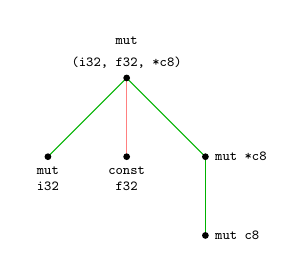
\begin{tikzpicture}

      \draw[-, black!30!green] (0,0) -- (-1,-1);
      \draw[-, red!50] (0,0) -- (0,-1);
      \draw[-, black!30!green] (0,0) -- (1,-1);
      \draw[-, black!30!green] (1,-1) -- (1,-2);

      \filldraw (0, 0.3) node[align=center, above] {\texttt{\tiny{mut}}};
      \filldraw (0, 0) circle (1pt) node[align=center, above] {\texttt{\tiny{(i32, f32, *c8)}}};
      \filldraw (-1,-1) circle (1pt) node[align=center, below]{\texttt{\tiny{mut}}};
      \filldraw (-1,-1.2) node[align=center, below]{\texttt{\tiny{i32}}};
      \filldraw (0,-1) circle (1pt) node[align=center, below]{\texttt{\tiny{const}}};
      \filldraw (0,-1.2) node[align=center, below]{\texttt{\tiny{f32}}};
      \filldraw (1,-1) circle (1pt) node[align=center, right]{\texttt{\tiny{mut *c8}}};
      \filldraw (1,-2) circle (1pt) node[align=center, right]{\texttt{\tiny{mut c8}}};


    \end{tikzpicture}
  }
  \caption{\label{fig:compound:tuple_mutability} Example of tuple mutability}
\end{figure}


The mutability level of inner types is only important when they are borrowing
data. In the previous example shown in Figure~\ref{fig:compound:tuple_mutability}, only
the mutability of the inner type \token{*c8} is important during data movement.
In other words, a value of type \token{mut (i32, f32, dmut *c8)} can be passed
to it without any problem. As with any borrowing type, the keyword
\token{alias} must be used when borrowing data.

\begin{lstlisting}[style=coloredverbatimError]
let mut x = 't'c8;
let mut a: mut (mut i32, f32, dmut *c8) = (1, 12.0f, &x);
let mut b: mut (i32, f32, dmut *c8) = (1, 7.0f, null);

a = alias b; // no problem
b = alias a; // no problem either

let c: (i32, f32, *c8) = (1, 7.0f, &x);
a = alias c; // not allowed, it would discard constant property of the third field
\end{lstlisting}

Tuple types with mutable values that don't borrow data are considered
non-borrowing types, and therefore don't need \token{alias} during data
movement. In practice, all the data of such a tuple is copied during data
movement.

The alignment of tuples follows the same rules as the alignment of structures
(see Chapter~\ref{chap:structures}): they are anonymous
structures.

\subsection{Properties}

Tuple type properties can be accessed by using the \token{::} operator on a
type expression. The properties are as follows:
\smallskip

\begin{center}
  \begin{adjustbox}{max width=\linewidth}
    \begin{tabular}{|l|ll|}
      \hline
      Name & Meaning & Type\\
      \hline
      \hline
      \token{init} & The initial value of the tuple, & \token{typeof(x)} \\
      & where every inner field is set to \token{T::init} & \\
      \Xhline{0.001pt}
      \token{arity} & The number of inner elements of the tuple type & \token{usize}\\
      \hline
      \token{typeid} & A string encoding the name of the type & \token{[c8]} \\
      \hline
    \end{tabular}
  \end{adjustbox}
\end{center}

\smallskip

Inner types are not accessible using the \token{::} operator, but are
accessible using \token{\_\_pragma}. Pragmas are presented in the
Section~\ref{sec:pragmas}.

\subsection{Binary operators}

Binary operators are divided into three groups:
\begin{itemize}
  \setlength\itemsep{-4pt}
\item Access: The operator \token{.} accesses a given field of the
  tuple. The right operand must be of type int and must be within the range of
  \token{0} and the arity of the tuple to be accessed. The result of the
  operation takes the type of the field at the index described by the right
  operand, and so does the value. The first field index is \token{0}.

  \begin{lstlisting}[style=coloredverbatimError, linewidth=0.95\linewidth]
let mut a: (mut i32, f32) = (8, 8.0f);

a.0 = 7; // allowed first field is mutable
a.1 = 1.0f; // not allowed, second field is not mutable

let c = a.(12 - 11); // accessing the field at index 1
  \end{lstlisting}

\item Comparison: The comparison operators \token{==} and \token{!=} are
  defined on tuples when each of the inner types are comparable. It compares all
  fields of two tuples and checks whether all inner values are equal for
  \token{==} or at least one inner value is different between the two operands
  for the operator \token{!=}.

  There is no relation of order between the tuples, even if they are of the same
  type, since in general such a comparison would be meaningless.

\item Assignment: The assignment operator creates a \textit{data movement}
  from the right operand to the left operand. Mutability must be respected when
  data is borrowed. Data mutability on tuples has already been introduced in
  Section~\ref{sec:compound:tuple_mutability}.

\end{itemize}

\subsection{Dollar operator}

The dollar operator can be used within an access binary operation in the right
operand expression. The dollar value takes the value of the arity of the tuple,
and its type is \token{usize}. Its value is known at compile time.

\begin{lstlisting}[style=coloredverbatim]
let a = (1, 9.0f, 'r');

let b = a.($ - 1us); // access the last value, i.e. 'r'
\end{lstlisting}

\subsection{Tuple expansion}

Tuples have a special operator called \token{expand} that turns them into a
list of parameters. Expanding a tuple is useful to create other tuples, or to
pass the data of the tuple as function parameters.

\begin{lstlisting}[style=coloredverbatim]
fn foo(a: i32, b: f32) {}

let a = (1, 5.0f);

 // transform a into a list of values
let b: (i32, f32, c32) = (expand a, 't');

foo(expand a); // transform a into a list of parameters
\end{lstlisting}

Such an operation is done at compile time and is simply a rewrite that is less
verbose. In fact, in the previous example, the line \token{foo(expand a)} is
rewritten as \token{foo(a.0, a.1)}. The mutability level of the expanded
values is always \token{1}, which means that tuple expansion can never borrow
mutable data. Tuple expansions are useful in variadic template functions to
write generic operations on a list of variadic parameters. The above example produces the following Ymir Intermediate Language code.

\begin{lstlisting}[style=myilVerb]
frame : main::main ()-> void {
    let a : (i32, f32) = (1, 5f);
    let b : (i32, f32, c32) = (a.0, a.1, 't'c32);
    main::foo (a.0, a.1);
    b;
    <unit-value>
}
\end{lstlisting}

\subsection{Tuple deconstruction}

A tuple declares several variables at once, using the same
\token{let} declaration. We call this declaration a tuple deconstruction
because it splits the values of the tuple into a list of variables. Types of
variables inside tuple deconstruction can be specified the same way they would
be specified for normal variable declaration. This defines more
complex levels of mutability.

\begin{lstlisting}[style=coloredverbatim]
  // a is mutable, but not b nor c
let (mut a, b, c) = (1, 't', 12.0f);

assert(a == 1 && b == 't' && c == 12.0f);

// With type specifications
let (mut d: i32, mut e: [mut f32 ; 2]) = (1, [1.0f, 2.0f]);
\end{lstlisting}

A variadic variable can be used as the last variable declaration in such a
deconstruction with the token \token{...}. In this case, it's type is always a
tuple that takes all the values in the tuple that are left and not associated
with other variables. The type of this last variable can be specified before the
token \token{...}.

\begin{lstlisting}[style=coloredverbatim]
let (a, b...) = (1, 2, 3);
assert(a == 1);
assert(b == (2, 3));

let (c, d...) = (1, 2);
assert(c == 1);
assert(d == (2,));

// With type specifications
let (e, f: (i32, f32)...) = (1, 2, 3.0f);
\end{lstlisting}

The above example produces the following Ymir Intermediate Language code. Notice
that in YIL, the tokens \tokennolst{\#\{} and \tokennolst{\#\}} declare a
set (a block of statements without lifetime). The variable lifetimes of \token{a}
and \token{b} are attached to the block declared by the function, not to the
set in which they are declared.

\begin{lstlisting}[style=myilVerb]
frame : main::main ()-> void {
    #{
        let a : i32 = 1;
        let b : (i32, i32) = (2, 3)
    #};
    core::exception::abort ((a == 1), (""s8)[]);
    core::exception::abort (((b.0 == 2) && (b.1 == 3)), (""s8)[]);
    #{
        let c : i32 = 1;
        let d : (i32,) = (2,)
    #};
    core::exception::abort ((c == 1), (""s8)[]);
    core::exception::abort ((d.0 == 2), (""s8)[]);
    #{
        let e : i32 = 1;
        let f : (i32, f32) = (2, 3f)
    #};
    <unit-value>
}
\end{lstlisting}

The mutability level of variables declared using tuple deconstruction can be
mutable by using the keywords \token{mut} or \token{dmut} on specific
variables of the tuple deconstruction (i.e. \token{let (dmut a, b) = alias
  t;}). In that case the right operand must match the mutability, and be aliased
explicitly.

\subsection{Tuple iteration}

Tuples are iterable types, allowing them to serve as the iterable value of a \token{for} loop.

\begin{lstlisting}[style=coloredverbatim]
let a = (1, 't', 89.0f);
for i in a {
    println(i);
}
\end{lstlisting}

In practice, because such an iteration would involve creating iterator variables
of different types, the iteration is unwound at compile time. The tuple value is
constructed only once before entering any loop body, resulting in the following
Ymir Intermediate Language code.

\begin{lstlisting}[style=myilVerb]
frame : main::main ()-> void {
    let a : (i32, c8, f32) = (1, 't'c8, 89f);
    cte for {
        {
            let i : i32 = 1;
            {
                std::io::println!{i32}::println (i);
                <unit-value>
            }
        };
        {
            let i : c8 = 't'c8;
            {
                std::io::println!{c8}::println (i);
                <unit-value>
            }
        };
        {
            let i : f32 = 89f;
            {
                std::io::println!{f32}::println (i);
                <unit-value>
            }
        }
    }
}
\end{lstlisting}

If two variables serve as iterators, the first indicates the iteration index,
and the second signifies the value within the tuple. However, in the case where
only one variable is specified, it exclusively contains the value of the tuple
field corresponding to the current iteration's index.

\begin{lstlisting}[style=coloredverbatim]
let dmut a = (1, 2, 3);
for i, _ in a {
    a.(i) = 9;
}

assert(a == (9, 9, 9));
\end{lstlisting}

More information about \token{for} loops is presented in Section~\ref{sec:flow:for_loops}.

\subsection{Implicit casting}

Tuple literal values may contain literal values that can be implicitly
converted during compilation (e.g. integer literals, array literals, class
objects, etc.). In this case, the conversion is performed at \token{cte}
implicitly.

\begin{lstlisting}[style=coloredverbatimError, escapechar=@]
// ok, '1' literal can be implicitly converted to '1us'
let mut a: (usize, usize) = (1, 2);

let mut i = 12;
a = @\hb{(i, i)}@; // error, 'i' is not cte, it cannot be converted to usize
\end{lstlisting}

This implicit casting is recursive and allowed for any inner values that might
be affected, but it only applies to tuple construction values, not to any tuple
values, even immutable ones.

\begin{lstlisting}[style=coloredverbatimError, escapechar=@]
// No problem, '0' is converted implicitly to '0us', and so on
let a: ([(usize, isize) ; 1], f32) = ([(0, 0)], 12.0);

// error, implicit cast is not allowed 'a' is not a tuple construction value
let b: ([(i32, i32) ; 1], f32) = @\hb{a}@;
\end{lstlisting}

\vfill%
\pagebreak

\section{Ranges}%
\label{sec:compound:range_type}

A range is a compound type consisting of four elements that describe a range of
values. The four elements are \token{fst} the first value of the range (e.g.
\token{0}), \token{scd} the last value of the range (e.g. \token{10}),
\token{step} the step of the range (e.g. \token{2}), and \token{contains} of
type bool, which indicates whether the last value \token{scd} is contained in
the range or not. There are only three types that can describe the inner
components of a range: integer, floating point and character. The type of the
range is defined by the inner type preceded by the token \token{..} (e.g.
\token{..i32} describes a range of \token{i32} values). Ranges are useful for
iteration or for accessing a subset of values (for example, a subset of a
slice).

\subsection{Literals}

Range literals are described using the \token{..} token or the \token{...}
token. The \token{..} token defines a range whose final value is not
included in the range, and the \token{...} token defines a range whose final
value is included. If different tokens describe the literal, the
type is the same, and the \token{..} token is always the only token used to
describe a range type.

\begin{lstlisting}[style=coloredverbatim]
let a: ..i32 = 0 .. 2;
let b: ..i32 = 0 ... 2;

cte assert(a.fst == b.fst);
cte assert(a.scd == b.scd);
cte assert(a.step == b.step);
cte assert(!a.contains && b.contains);
\end{lstlisting}

Range values can be decreasing, in which case the step is negative. Note that
for ranges of unsigned integers and character values, it is theoretically
impossible to have a negative value for the step. The overflow behaviour of
those types is used instead, to create a value that, when added to
\token{fst}, equals \token{fst - abs(step)} (at the binary level this is
exactly the same as adding a negative value, even though it is not a valid high
level representation). For this reason the step can be
considered to always be a signed version of the type, even if the field
type is considered to be the same as the type of the inner values (\token{fst}
and \token{scd}), and thus one bit of its encoding is always used for the sign.
\smallskip

The \token{fst} value of the range literal is constructed before the
\token{scd} value. In the following example, the function \token{foo} is
called before the function \token{bar}.

\begin{lstlisting}[style=coloredverbatim]
fn foo()-> i32 {
  println("In foo.");
  12
}

fn bar()-> i32 {
  println("In bar.");
  1
}

let a = (foo()) .. (bar());
println(a);
\end{lstlisting}

\subsection{Mutability and memory alignment}

As one might expect, range values do not share any data, and every field
included in the value is replicated during data movement. Therefore, there is no
concern for mutability, rendering the type not aliasable. A mutable range has
the ability to modify its internal fields, but even if the range type is a
compound type, it operates precisely like a scalar type since it can never
contain any borrowed data. In memory a range value has the same memory
alignment as the structure (cf. Chapter~\ref{chap:structures}) presented in the
following source code where \token{T} is the inner type of the range.

\begin{lstlisting}[style=coloredverbatim]
record Range {T} {
  let fst: T;
  let scd: T;
  let step: T;
  let contains: bool;
}
\end{lstlisting}

\subsection{Properties}

Range type properties can be accessed through the operator \token{::} applied
to a type expression. The properties are as follows:

\begin{center}\begin{adjustbox}{max width=\linewidth}
  \begin{tabular}{|l|ll|}
    \hline
    Name & Meaning & Type\\
    \hline
    \hline
    \token{init} & The initial value ranging from \token{T::init} & \token{typeof (x)}\\
    & to \token{T::init} with a step of \token{T::init} and & \\
    & with \token{contains} set to \token{false} where \token{T} is & \\
    & the inner type (e.g. \token{i32} for \token{..i32}). &\\
    \hline
    \token{typeid} & A string encoding the name of the type & \token{[c8]} \\
    \hline
  \end{tabular}
\end{adjustbox}\end{center}


\subsection{Binary operators}

Binary operators are divided into four groups:

\begin{itemize}
  \setlength\itemsep{-4pt}
\item Access: The operator \token{.} is utilized to access the field of the
  range type. The right operand is the name of the field to access. The fields
  are listed in the table below.

  \begin{center}\begin{adjustbox}{max width=\linewidth}
    \begin{threeparttable}
      \begin{tabular}{|l|ll|}
        \hline
        Name & Value & Type\\
        \hline
        \hline
        \texttt {fst} & The first value of the range & \textit{T}$^{1^{\phantom{j}}}$ \\
        \texttt {scd} & The last value of the range & \textit{T}$^{1^{\phantom{j}}}$ \\
        \texttt {step} & The step of the range & \textit{S}$^{2^{\phantom{j}}}$ \\
        \texttt {contains} & The field describing whether or not & \token{bool} \\
        & the \token{scd} value is contained in the range &\\
        \hline
      \end{tabular}
      \begin{tablenotes}
      \item[1.] \token{__pragma!inner (typeof (x), 0)}
      \item[2.]\small \textit{Signed version of inner type for integer type
        ranges, an integer type for character type ranges, and
        \token{__pragma!inner (typeof(x), 0)} for float type ranges.}
      \end{tablenotes}
    \end{threeparttable}
\end{adjustbox}\end{center}

Accessed fields are only mutable if the range is also mutable.

\item Contains: The \token{in} and \token{!in} operators verify the presence
  of a value in a range. The left operand must match the inner type of the right
  operand, and the right operand must be a range type.

\item Comparison: Ranges can be compared using the operators \token{==} and
  \token{!=}. This checks the equality or inequality of each field within the
  range. The left and right operands must be of the same type.

\item Assignment: A range value can be an lvalue if and only if it is mutable.
  \begin{lstlisting}[style=coloredverbatim]
let mut a = 0 .. 7;

a = 7 .. 1;
  \end{lstlisting}

\end{itemize}

\subsection{Implicit casting}

Unlike tuple, array, slice and option literals, the values of a range literal
are not implicitly converted at \token{cte}. The inner type of the range is
always the type of its operands, so a literal whose operands are of a different
type than the expected one is an error, even when its operands are known at
compile time.

\begin{lstlisting}[style=coloredverbatimError]
let a: ..usize = 0us .. 2us; // ok, the operands are already usize

let b: ..usize = 0 .. 2; // error, '0' and '2' are i32 literals
\end{lstlisting}

\subsection{Range iteration}

 Ranges are iterable types, so they can be used as the iterable value of a
 \token{for} loop. Only one immutable variable can be declared when iterating
 over a range value. This iterator variable takes the value of the \token{fst}
 field of the range and increments by the \token{step} field until it reaches
 the \token{scd} field. If the range is a containing range (i.e. the
 \token{contains} field is true), then the \token{scd} field is included in
 the iteration. Optimisations are performed if the inner values of the range are
 known at compile time.

\begin{lstlisting}[style=coloredverbatim]
for i in 0 .. 7 {
    print(i, ' '); // 0 1 2 3 4 5 6
}

for i in 0 ... 7 {
    print(i, ' '); // 0 1 2 3 4 5 6 7
}

for i in 7 .. 0 {
    print(i, ' '); // 7 6 5 4 3 2 1
}
\end{lstlisting}

For more information on \token{for} loops, see the Section~\ref{sec:flow:for_loop}.

\vfill%
\pagebreak

\section{Arrays}%
\label{sec:compound:arrays}

 An array is a compound type containing a list of values of the same type stored
 in a contiguous memory segment and whose size is known at compile time. An
 array type is described using the following syntax \token{[T ; N]} where
 \token{T} is the inner type of the array and \token{N} is an integer value
 describing the number of elements contained in the array.

\subsection{Literals}

Array literals are a list of values enclosed in brackets \token{[} and
  \token{]}. An array literal of size \token{0} contains no data and consists
only of the brackets, its type is always \token{[void ; 0]}, and it can be
assigned to any lvalue with an array type whose size is \token{0}.

\begin{lstlisting}[style=coloredverbatim]
fn foo(x: [i32 ; 4]) {
  println(x);
}

let a = [1, 2, 3]; // array [i32 ; 3]
let b: [i32 ; 3] = [1, 2, 3]; // array [i32 ; 3]

foo([1, 2, 3, 4]); // calling with an array [i32 ; 4]

let c: [i32 ; 0] = []; // ok, [void ; 0] can be implicitly cast to [i32 ; 0]

println(a, " ", b);
cte assert(c.len == 0us);
\end{lstlisting}

Array inner values are constructed in the order they are written. In the
following example, the function \token{foo} is called before the function
\token{bar}.

\begin{lstlisting}[style=coloredverbatim]
fn foo()-> i32 {
  println("In foo.");
  1
}

fn bar()-> i32 {
  println("In bar.");
  2
}

let a: [i32 ; 2] = [foo(), bar()];
println(a);
\end{lstlisting}

There are two other ways to define an array literal value. The first is the
array construction syntax. This syntax is similar to the type description of the
type array, but uses a value instead of a type \token{[V ; N]}. Each element of
the array takes the value \token{V}. When this syntax is used, the inner value
is constructed only once and replicated at each index of the array. In the
following example, the function \token{foo} is called once and each index of
the array contains the value \token{12}.

\begin{lstlisting}[style=coloredverbatim]
fn foo()-> i32 {
  println("In foo.");
  12
}

let a = [foo() ; 4];
println(a); // [12, 12, 12, 12], after a single "In foo."
\end{lstlisting}

\smallskip
The last array literal syntax uses a \token{for} loop. This syntax, called list
comprehension, is explained in more detail in the Section~\ref{sec:compr:list_compr}.
Unlike the array construction syntax, the values are calculated at each index of
the array, so the function is called four times in the following code, when it
would have been called only once using the array construction syntax.

\begin{lstlisting}[style=coloredverbatim]
fn foo()-> i32 {
  println("In foo.");
  12
}

let a = [foo() for _ in 0 .. 4];
assert(a[0] == a[1]);
\end{lstlisting}


\subsection{Mutability and memory alignment}
Arrays do not borrow data because they store data as the actual list of values
contained in the array. Therefore, when data is moved, all the data in the array
is copied. The mutability level of an array is only important if the inner type
of the array borrows data, similar to tuples. Figure~\ref{fig:compound:data_repr_array}
shows the memory representation of the following example.

\begin{lstlisting}[style=coloredverbatimError]
let dmut a: [i32 ; 3] = [1, 2, 3];

let dmut b = a; // no need for alias
                // a and b don't refer to the same memory segment

let i = 89;
let c: [*i32 ; 1] = [&i];

let dmut d = c; // not allowed, discard const property of the inner type
\end{lstlisting}

\begin{figure}[h]
  \centering
  \begin{adjustbox}{max width=\linewidth}
    \begin{tikzpicture}
      \foreach \name/\y/\base/\values in {a/0/0/{1, 2, 3}, b/-1.4/12/{1, 2, 3}} {
        \foreach \value [count=\i from 0] in \values {
          \pgfmathtruncatemacro{\at}{\base + 4 * \i}
          \node[memcell] (\name\i) at (\i * 1.0, \y) {\value};
          \node[memnote, above=0.5mm of \name\i] {+\at};
        }
      }
      \node[memcell] (i) at (0, -2.8) {89};
      \node[memnote, above=0.5mm of i] {+24};
      \node[memcell, fill=black!8, right=0mm of i] (pad) {};
      \node[memnote, above=0.5mm of pad] {+28};
      \node[memnote, right=1mm of pad] (padn) {padding};
      \node[memaddr, minimum width=20mm] (c) at (0.5, -4.2) {};
      \node[memnote, anchor=south] at ([xshift=5mm, yshift=0.5mm]c.north west) {+32};
      \node[cflab, left=3mm of a0] (an) {\token{a}};
      \node[cflab, left=3mm of b0] {\token{b}};
      \node[cflab, left=3mm of i] {\token{i}};
      \node[cflab, left=3mm of c] (cn) {\token{c}};
      \node[memframe, fit=(an)(a2)(padn)(cn)(c), inner ysep=4mm] (foo) {};
      \node[memtitle] at ([xshift=2mm]foo.north west) {foo};
      \draw[mempoint] ([xshift=-5mm]c.center) -- (i.south);

      \node[memregion] at ($(foo.north) + (0, 5mm)$) {stack};
    \end{tikzpicture}
  \end{adjustbox}
  \caption{\label{fig:compound:data_repr_array} The frame of \token{foo}, with
    the offset of each word above it. The arrays \token{a} and \token{b} each
    hold their three elements, 12 bytes, so \token{b} is a copy that shares
    nothing with \token{a}. \token{c}, an array of one pointer, is aligned on
    8 bytes after the 4 bytes of \token{i}, and borrows \token{i}.}
\end{figure}


\subsection{Properties}

Array type properties can be accessed using the \token{::} operator on a type
expression. The properties are as follows:

\begin{center}\begin{adjustbox}{max width=\linewidth}
  \begin{tabular}{|l|ll|}
    \hline
    Name & Meaning & Type\\
    \hline
    \hline
    \token{init} & The initial value, where all inner & \token{typeof(x)} \\
    & values are set to \token{T::init}, \token{T} being & \\
    & the inner type of the array & \\
    \Xhline{0.001pt}
    \token{size} & The static size of the array (is equal to \token{.len}) & \token{usize} \\
    \hline
    \token{typeid} & A string encoding the name of the type & \token{[c8]} \\
    \hline
  \end{tabular}
\end{adjustbox}\end{center}

\subsection{Binary operators}

Binary operators are divided into four groups:

\begin{itemize}
  \setlength\itemsep{-4pt}
\item Access: The \token{.} operator accesses fields that describe the
  array value. The right operand is the name of the field to be accessed. These
  fields are described in the table below.

  \begin{center}\begin{adjustbox}{max width=\linewidth}
      \begin{threeparttable}
        \begin{tabular}{|l|ll|}
          \hline
          Name & Value & Type\\
          \hline
          \hline
          \token{len} & The size of the array & \token{usize} \\
          \token{ptr} & The pointer to the first element  & \textit{T}$^{1^{\phantom{J}}}$\\
          & of the array & \\
          \hline
        \end{tabular}
        \begin{tablenotes}
        \item [1.] inner type of the array, i.e. \token{*(__pragma!inner (typeof (x), 0))} \\
        \end{tablenotes}
      \end{threeparttable}
\end{adjustbox}\end{center}

The \token{len} field is known at compile time and can therefore be used in
a \token{cte} expression. The type of the \token{ptr} field has the same
level of mutability as the array type. Note that array does not really have
fields. The values are constructed from the array information, \token{ptr}
takes the address of the array as a value, and \token{len} is an integer
literal containing the length of the array in number of elements contained.

\item Concatenation: The concatenation operator \token{\~} creates an
  array or slice containing the values of two arrays or slices. The operator can
  be used if the left and right operands have the same internal type, regardless
  of their relative sizes. The mutability of the generated value is the
  strictest mutability between the two operands. For example, the type and
  mutability of \token{([*i32 ; 4]) \~\ (dmut [*i32 ; 2])} is \token{[*i32 ;
      6]} to avoid discarding the constant property of the values contained in
  the left operand. Notice that the type of the generated value is an array
  whose size is the sum of the left and right operand sizes.

  The operator can also be used when one of the operands is a slice. In this
  case, the return value of the operation will be a slice instead of an array,
  since its size cannot be known at compile time. This operation is actually
  performed more by the slice operand than by the array operands, and is
  discussed further in Section~\ref{sec:compound:slices}.

  The operator \token{\~} was chosen to avoid confusion with \token{+}, which
  would behave differently depending on the operands. Concatenation is not really
  an arithmetic operation, as \token{+} would refer to an addition of all the
  inner values of two arrays, rather than their concatenation. Concatenation
  operator is obviously not commutative.

  \begin{lstlisting}[style=coloredverbatim]
let a: [i32 ; 3] = [1, 2, 3];
let b: [i32 ; 2] = [4, 5];

let c: [i32 ; 5] = a ~ b;

assert(c == [1, 2, 3, 4, 5]);
  \end{lstlisting}

\item Comparison: Binary comparison operators can be used with two arrays of the
  same inner type, or an array and a slice of the same inner type. The result of
  the operation is always of type \token{bool}. For the operators to work, the
  inner type of the array must also define the comparison operators. Lexical
  order is used, so the size of the arrays is only used if one of the two operands
  is a prefix of the other (e.g. \token{[1, 2]} is a prefix of \token{[1, 2,
      3]}, so \token{[1, 2, 3]} is considered greater than \token{[1, 2]}, but
  \token{[1, 3]} is greater than \token{[1, 2, 3]}).

  \begin{center}\begin{adjustbox}{max width=1.0\linewidth}
    \begin{tabular}{|c|lll|}
      \hline
      Operator & Operation & Comm. & Example\\
      \hline
      \hline
      \token{>}      & Greater than     & No          & \token{([1, 2] > [2, 3]) == false}    \\
      \token{<}      & Lower than       & No          & \token{([1, 2] < [2, 3]) == true}     \\
      \token{>=}     & Greater or equal & No          & \token{([1, 2, 3] >= [1, 2]) == true} \\
      \token{<=}     & Lower or equal   & No          & \token{([1, 2, 3] <= [2]) == true}    \\
      \token{==}     & Equal            & Yes         & \token{([1, 2] == [1, 2]) == true}    \\
      \token{!=}     & Not equal        & Yes         & \token{([1, 2] != [1, 2]) == false}   \\
      \hline
    \end{tabular}
  \end{adjustbox}\end{center}

\item Assignment: An array value can be an lvalue if and only if it is mutable.
  Information about inner type mutability has already been discussed in the
  section on mutability, and will therefore not be discussed further here. The
  size of the left and right operands must of course be strictly equal.

  \begin{lstlisting}[style=coloredverbatim]
let mut a: [i32 ; 2] = [1, 2];

a = [2, 3];
  \end{lstlisting}

\end{itemize}

\subsection{Index operator}

The index operator can be used on an array as the left operand, with an int
value or a range value as the right operand.

\begin{itemize}
  \setlength\itemsep{-4pt}
\item With an int value: the element at the index described by the int value is
  returned. The mutability of the result value depends on the mutability of the
  inner type of the array. If the mutability level of the array type is at least
  \token{2}, the result value can be used as lvalue.

  \begin{lstlisting}[style=coloredverbatimError]
let mut a: [mut i32 ; 3] = [1, 2, 3];
let mut b: [i32 ; 2] = [4, 5];

a[0] = 9; // ok, mutability level of 'a' is high enough

b[0] = 11; // not allowed, b inner values are not mutable
b = [9, 10]; // ok, b is mutable
  \end{lstlisting}

  If the value of the int operand is known at compile time, a size check is
  performed to ensure that the access does not overflow the array size, and that
  the value used is greater than or equal to zero. If the value is unknown at
  compile time, a condition is added and an array size check is performed at
  runtime. Panic is triggered if an overflow occurs.

  In the first version of Ymir, the exception
  \token{core::exception::OutOfArray} was thrown, which forced developers to
  deal with the exception. This made the program extremely strict, forcing the
  developer to double check every array access by hand. Programming became
  relatively impractical. Developers generally responded to this problem with
  control flow \token{try \{ \} catch \{ panic; \}}. Thus, a faster
  compiler-generated approach was chosen (i.e., \token{if (out) panic;}). This
  test is turned off if the compiler can ensure the inbound test without knowing
  the exact value of the index.

\item With a range value: using a range value containing int values as the right
  operand, the program creates a slice containing only a subset of the array
  values. The mutability level of the created slice type is the same as the
  mutability of the array type. The \token{copy} operator must be used to create
  the slice value, as it allocates memory on the heap (see Slice
  limitation~\ref{sec:compound:slice_lim}) and to prevent implicit memory allocations.

  \begin{lstlisting}[style=coloredverbatim]
let a: [i32 ; 4] = [1, 2, 3, 4];

let b: [i32] = copy a[0 .. 2];
println(b); // [1, 2]
  \end{lstlisting}

  If the inner values of the range are known at compile time, it is checked that
  there will be no array overflow. The range must be ascending, i.e. the first
  value of the range must be less than the second value. This is also checked at
  compile time if possible. If the values of the range are not known at compile
  time, then these checks are done at runtime. The \token{contains} field of the range
  has no effect on the array access, and the \token{scd} value is always
  considered not contained.

  If the range used to index the array is known at compile time, a new array
  value can be created. In that case the \token{copy} operator is no longer
  mandatory, and the result of the operand is an array value.

  \begin{lstlisting}[style=coloredverbatim]
fn foo(a: [i32 ; 3]) {
  println(a);
}

let a = [1, 2, 3, 4];
foo(a[1 .. 4]);
  \end{lstlisting}

\end{itemize}

\subsection{Dollar operator}

The dollar operator can be used within an index operation in the right operand
expression. The dollar value takes the value of the size of the array and its
type is \token{usize}. Its value is known at compile time.

\begin{lstlisting}[style=coloredverbatim]
let a: [i32 ; 4] = [1, 2, 3, 4];

let b = a[0us .. $ - 1us]; // all the values except the last one

let c = a[$ - 2us]; // the second-to-last value

println(b, ' ', c); // [1, 2, 3] 3
\end{lstlisting}

\subsection{Array iteration}

Arrays are iterable types, so they can be used as iterable values of a
\token{for} loop. The \token{for} loop can use either one or two variables as
iterators. If a single variable is used, it automatically captures the value of
the array element at the current iteration index. Conversely, if two variables
are used, the first variable represents the iteration index, while the second
variable stores the value of the array element at that specific index.

\begin{lstlisting}[style=coloredverbatim]
let a: [i32 ; 4] = [1, 2, 3, 4];
for i, elem in a {
    assert(a[i] == elem);
}

// Only 1 iterator, captures the value
for elem in a {
  print(elem, ' '); // 1 2 3 4
}
\end{lstlisting}

In practice, a slice is created over the array value (without copying) to ensure
that the array is created only once. Thus, the above code is rewritten as
follows by the compiler. This code is not valid Ymir source code, but a
representation of what the compiler generates before performing optimizations.

\begin{lstlisting}[style=myilVerb]
let mut a : mut [mut i32 ; 4us] = [1, 2, 3, 4];
{
  let #_value : [mut i32] = {.len = 4us, .ptr = &a[0]};
  let elem : i32;
  let i : usize = 0us;
  while (i < #_value.len) {
    elem = #_value [i];
    {
      core::exception::abort (a [i] == elem, (""s8)[]);
      <unit-value>
    };
    i = (i + 1us)
  }
}
\end{lstlisting}


\subsection{Array expansion}

The special operator \token{expand} can be used on arrays, to turn them into a
list of parameters. This operator passes the values of an array as
function parameters, or to construct another array, or even a tuple.

\begin{lstlisting}[style=coloredverbatim]
fn foo(a: i32, b: i32) {
  println(a, " ", b);
}

let a: [i32 ; 2] = [1, 2];
let b: [i32 ; 3] = [expand a, 3];

foo(expand a);

let c: (i32, i32, i32) = (expand b,); // the trailing comma is mandatory, it is a tuple literal
println(c);
\end{lstlisting}

This operation is done at compile time and is simply a less verbose rewrite. In
fact, in the previous example, the line \token{foo(expand a)} is rewritten as
\token{foo(a[0], a[1])}. The mutability level of the expanded values is
always \token{1}, i.e. array expansion can never borrow mutable data. This
operation can be done because the size of an array is known at compile time. The
above example produces the following Ymir Intermediate Language code.

\begin{lstlisting}[style=myilVerb]
frame : main::main ()-> void {
    let a : [i32 ; 2us] = [1, 2];
    let b : [i32 ; 3us] = [a [0us], a [1us], 3];
    main::foo (a [0us], a [1us]);
    let c : (i32, i32, i32) = (b [0us], b [1us], b [2us]);
    c;
    <unit-value>
}
frame : main::foo (a : i32, b : i32)-> void {
    a;
    b;
    <unit-value>
}
\end{lstlisting}


\subsection{Implicit casting}

Array literal values may contain literal values that can be implicitly
converted during compilation (e.g. integer literals, tuple construction values,
class objects, etc.). In this case, the conversion is performed at \token{cte}
implicitly.

\begin{lstlisting}[style=coloredverbatimError, escapechar=@]
// ok, '1' literal can be implicitly converted to '1us'
let mut a: [usize ; 2] = [1, 2];

let mut i = 12;
// error, 'i' is not cte, it cannot be converted
a = @\hb{[i, i]}@;
\end{lstlisting}

This implicit casting is recursive and allowed for any inner values that might
be affected, but it only applies to array literal values, not to any array
values, even immutable ones.

\begin{lstlisting}[style=coloredverbatimError, escapechar=@]
// No problem, '0' is converted implicitly to '0us', and so on
let a: [(usize, isize) ; 2] = [(0, 8), (1, 2)];

// error, implicit cast is not allowed, 'a' is not an array literal
let b: [(i32, i32) ; 2] = @\hb{a}@;
\end{lstlisting}

\subsubsection{Implicit conversion of string literal}

String literals (see Section~\ref{sec:string_lit}) can be converted to array
values at compile time. String literals live in the text segment, and are
thus pointers to it, hence their proximity to the slice type. However, since their
values are actually known at \token{cte}, they can be converted to array
literal values. This conversion is done implicitly using an array type value as
lvalue and a \token{cte} string literal value as rvalue.

\begin{lstlisting}[style=coloredverbatim]
let a: [c32 ; 5] = "Hello";
let b: [c8 ; 5] = "Hello"; // no need for suffix, implicit char conversion is allowed on cte values

println(a, ' ', b); // [H, e, l, l, o] [H, e, l, l, o]
\end{lstlisting}

The program's behavior differs when using array values stored on the stack
compared to using slices. In this case, the program uses 25 bytes of memory on
the stack, whereas slices would have used 48 bytes on a 64-bit system. This is
because the array values use 5 times 4 bytes (for the \token{c32} array) plus 5
bytes (for the \token{c8} array), while a slice value is three words long (see
Section~\ref{sec:compound:slices}). For big string literals, it has to be taken into
account.

\vfill%
\pagebreak

\section{Slices}%
\label{sec:compound:slices}

A slice is a compound type that contains a list of values of the same type that
are stored in a contiguous segment of memory, but the size of which is unknown
at compile time. A slice is described using the syntax \token{[T]}, where
\token{T} is the inner type of the slice. Unlike array types, slices are
pointers to borrowed memory, and are allocated on the heap, or written in the
text segment (e.g. string literals).

In practice, a slice is a pointer \token{*T} to the borrowed data, a
\token{usize} storing the size of the slice, and a third word holding the
metadata of the memory block the data belongs to, used when appending values to
the slice. A slice value is therefore 24 bytes long on a 64-bit system. A slice
may contain no data, in which case both the pointer and the size are equal to
\token{0}. If the size of the slice is strictly positive, then the pointer is
non-null. The block metadata may be null even when the slice is not empty, in
which case appending to the slice reallocates it.


\begin{figure}[h]
  \centering
  \begin{adjustbox}{max width=\linewidth}
    \begin{tikzpicture}
      \node[memcell] (xlen) at (0, 0) {3};
      \node[memaddr, right=0mm of xlen] (xptr) {};
      \node[memcell, right=0mm of xptr] (xblk) {\dots};
      \foreach \field/\off in {len/0, ptr/8, blk/16} {
        \node[memnote, above=0.5mm of x\field] {\field\ +\off};
      }
      \node[cflab, left=3mm of xlen] (xn) {\token{x}};
      \node[memframe, fit=(xn)(xblk), inner ysep=4mm] (foo) {};
      \node[memtitle] at ([xshift=2mm]foo.north west) {foo};

      \foreach \value [count=\i from 0] in {1, 2, 3} {
        \node[memcell] (h\i) at (6.4 + \i * 1.0, -0.6) {\value};
      }
      \node[memnote, above=0.5mm of h0] {0xfa45b987};
      \draw[mempoint] (xptr.center) .. controls +(0, -1.0) and +(-1.5, 0) .. (h0.west);

      \node[memregion] (stack) at ($(foo.north) + (0, 5mm)$) {stack};
      \node[memregion] at (h1 |- stack.base) {heap};
      \draw[memsep] (5.2, 1.4) -- (5.2, -1.2);
    \end{tikzpicture}
  \end{adjustbox}
  \caption{\label{fig:compound:data_repr_slice} The slice
    \token{x = copy [1, 2, 3]} in the frame of \token{foo}: a length, a pointer
    to the elements on the heap, and the block metadata, one word each.}
\end{figure}


\subsection{Literals}

There is no literal syntax that builds a slice from a list of values. Such a
list is always an array literal (see Section~\ref{sec:compound:arrays}), and becomes a
slice only through the \token{copy} or \token{dcopy} operator, for the reason
given in the following subsection. Two literals are nonetheless slice values.

The first is the empty literal \token{[]}, which borrows no memory and can
therefore be given a slice type without \token{copy}. The second is the string
literal, which resides in the text segment and is thus already a pointer to
borrowed memory. A string literal with no suffix has the type \token{[c8]}; the
suffixes \token{s8} and \token{s32} give the types \token{[c8]} and
\token{[c32]} respectively. Because the text segment is immutable, a string
literal can never be given a mutable slice type, \token{copy} must be used to
obtain one.

\begin{lstlisting}[style=coloredverbatimError]
let a: [i32] = []; // ok, an empty slice borrows nothing
let b: [c8] = "Hello"; // ok, a string literal is already a slice
let c: [c32] = "Hello"s32;

let dmut d: [c8] = "Hello"; // not allowed, the text segment is immutable
let dmut e: [c8] = copy "Hello"; // ok
\end{lstlisting}

\subsection{Limitation}%
\label{sec:compound:slice_lim}

Because a slice can be created from an array value, it can point to nowhere.
This is a big problem, and it does not seem to be solvable by static analysis.

%% check: skip -- hypothetical: shows the unsafe program the copy rule prevents
\begin{lstlisting}[style=coloredverbatim]
fn foo(a: [i32])-> [i32] {
    a
}

fn bar()-> [i32] {
    let a: [i32 ; 2] = [1, 2]; // 'a' does not exist at the end of bar

    foo(a) // but is returned from this function call
}

let x = bar();
println(x); // undefined behavior
\end{lstlisting}

Forcing the copy of the array when creating a slice from it seems to be the only
reasonable way to solve this problem. This means that slices never point to
memory on the stack, but always to the heap. The same limitation exists for
pointers, but pointers are not intended to be used outside of
trusted and unsafe parts of code, where slices are one of the most common types,
and restricting their operations to unsafe contexts only would be extremely
limiting.

\begin{lstlisting}[style=coloredverbatimError]
let a: [i32 ; 2] = [1, 2];
let b: [i32] = a; // not allowed
let c: [i32] = copy a; // ok
\end{lstlisting}



\subsection{Mutability and memory alignment}

Slices borrow data (that resides on the heap, or in an immutable memory segment
such as the text segment), so when moving data it is important to consider the mutability of the
borrowed data. Slices have three levels of mutability, 0, 1 and 2, where 0 means
that neither the slice nor the inner data is mutable, 1 means that the slice is
mutable but not the inner data, and finally 2 means that both the slice and the
inner data are mutable. The mutability level can of course be recursive if the
slices contain borrowed data.


As an example to illustrate the memory representation of slices, the
Figure~\ref{fig:compound:data_repr_slice} shows the memory representation of the slice
value \token{x = copy [1, 2, 3]}. Slices with a mutability level of 2
cannot be moved or copied without explicit specification. The keywords
\token{alias}, \token{copy} and \token{dcopy} must be used, as specified in
Section~\ref{sec:memory:memory_movement}.

\begin{lstlisting}[style=coloredverbatimError]
let dmut a: [[i32]] = copy [copy [1], copy [2], copy [3]];

let dmut b = a; // forbidden
let dmut c = alias a; // ok, make a reference to the same data as 'a'
let dmut d = copy a; // forbidden copy of 'a' is 'mut [mut [i32]]', not 'mut [mut [mut i32]]'

let dmut e = dcopy a; // ok, deeply copy of 'a'
\end{lstlisting}



\subsection{Properties}

The properties of a slice type can be accessed by using the \token{::} operator on a type expression. The properties are:

\begin{center}\begin{adjustbox}{max width=\linewidth}
  \begin{tabular}{|l|ll|}
    \hline
    Name & Meaning & Type\\
    \hline
    \hline
    \token{init} & The initial value & \token{typeof(x)}\\
    & an empty slice of size \token{0} & \\
    \hline
    \token{typeid} & A string encoding the name of the type & \token{[c8]} \\
    \hline
  \end{tabular}
\end{adjustbox}\end{center}

\subsection{Binary operators}

Binary operators are divided into four groups:
\begin{itemize}
  \setlength\itemsep{-4pt}
\item Access: The operator \token{.} accesses fields that describe the slice value. The right operand is the name of the field to be accessed. These fields are described in the table below.

  \begin{center}\begin{adjustbox}{max width=\linewidth}
      \begin{threeparttable}
        \begin{tabular}{|l|ll|}
          \hline
          Name & Value & Type\\
          \hline
          \hline
          \token{len} & The size of the slice & \token{usize} \\
          \token{ptr} & The pointer to the first element  & \textit{T}$^{1^{\phantom{j}}}$ \\
          & of the slice & \\
          \hline
        \end{tabular}
        \begin{tablenotes}
        \item [1.] inner type of the slice, i.e. \token{*(__pragma!inner (typeof (x), 0))} \\
        \end{tablenotes}
      \end{threeparttable}
  \end{adjustbox}\end{center}

  The type of the \token{ptr} field has the same level of mutability as the
  slice type. The \token{len} field contains the number of elements contained
  in the data borrowed by the slice.

\item Concatenation: The concatenation operator \token{\~} creates a
  slice containing the values of two slices, or an array and a slice. The
  operator can be used if the left and right operands have the same internal
  type, regardless of their relative sizes. The mutability of the generated
  value is the strictest mutability between the two operands. For example, the
  type and mutability of \token{([*i32]) \~\ (dmut [*i32])} is \token{[*i32]}
  to avoid discarding the constant property of the values contained in the left
  operand. Unlike array concatenation, this operator allocates memory on the
  heap whenever a slice is involved as at least one of the two operands.
  Concatenation operator is obviously not commutative.

\item Comparison: Binary comparison operators can be used with two slices of the
  same inner type, or a slice and an array whose inner types are comparable. The
  result of the operation is always of type \token{bool}. For the operators to
  work, the inner type of the slice must also define the comparison operators.
  Lexical order is used, so the size of the slices is only used if one of the
  two operands is a prefix of the other (e.g. \token{[1, 2]} is a prefix of
  \token{[1, 2, 3]}, so \token{[1, 2, 3]} is considered greater than
  \token{[1, 2]}, but \token{[1, 3]} is greater than \token{[1, 2, 3]}).

  \begin{center}\begin{adjustbox}{max width=1.0\linewidth}
    \begin{tabular}{|c|lll|}
      \hline
      Operator & Operation & Comm. & Example\\
      \hline
      \hline
      \token{>}      & Greater than     & No          & \token{([1, 2] > [2, 3]) == false}    \\
      \token{<}      & Lower than       & No          & \token{([1, 2] < [2, 3]) == true}     \\
      \token{>=}     & Greater or equal & No          & \token{([1, 2, 3] >= [1, 2]) == true} \\
      \token{<=}     & Lower or equal   & No          & \token{([1, 2, 3] <= [2]) == true}    \\
      \token{==}     & Equal            & Yes         & \token{([1, 2] == [1, 2]) == true}    \\
      \token{!=}     & Not equal        & Yes         & \token{([1, 2] != [1, 2]) == false}   \\
      \hline
    \end{tabular}
  \end{adjustbox}\end{center}

\item Assignment: A slice value can be an lvalue if and only if it is mutable.
  The size of the left and right operands is irrelevant during slice
  assignment. Slice assignment represents a memory movement, so the mutability
  of the inner values is important. Indeed, if the mutability level of the left
  operand is higher than the mutability level of the right operand, then the
  constant property would be discarded, removing its guarantee, so it is not
  allowed.

  \begin{lstlisting}[style=coloredverbatimError]
let      a = copy [1, 2, 3]; // const [i32]
let dmut b = copy [2, 3, 4]; // mut [mut i32]
let dmut c = copy [5, 9]; // mut [mut i32]

a = copy [2, 3]; // not allowed, 'a' is const
b = a; // not allowed, discard const property of inner values of 'a'
b = c; // not allowed, implicit alias
b = alias c; // ok
  \end{lstlisting}

\end{itemize}


\subsection{Index operator}

The index operator can be used on a slice value as the left operand, with an int
value or a range value as the right operand.

\begin{itemize}
  \setlength\itemsep{-4pt}
\item With an int value: the element at the index described by the int value is
  returned. The mutability of the result value depends on the mutability level
  of the inner type of the slice. If the mutability level of the slice type is
  at least \token{2}, the result value can be used as lvalue.

  \begin{lstlisting}[style=coloredverbatimError]
let dmut a = copy [1, 2, 3];
let mut  b = copy [4, 5];

a[0] = 9; // ok, mutability level of 'a' is high enough
b[0] = 11; // not allowed, b inner values are not mutable
b = copy [9, 10]; // ok, b is mutable
  \end{lstlisting}

  Since the size of the slice value is not known at compile time (most of the
  time), a condition is added at runtime and a size check is performed to ensure
  that the index is valid. A panic is triggered if an overflow occurs. Sometimes
  the size of the slice can be inferred, or the order inequality between the
  index and the size of the slice can be guaranteed, in these cases the size
  check is done at compile time and no condition is added at runtime.

\item With a range value: using a range value containing int values as the right
  operand, the program creates a slice containing only a subset of the slice
  value. The mutability level of the created slice is the same as the mutability
  level of the left operand of the operation. Unlike the array index operator
  with a range, no \token{copy} operator is mandatory. In fact, the memory
  borrowed by a slice value is always on the heap, so the risk presented in
  Section~\ref{sec:compound:slice_lim} is not present when dealing only with slices. Such
  an index operator does not copy any memory, it only creates a new reference,
  no implicit memory allocation takes place.

  \begin{lstlisting}[style=coloredverbatim]
let a = copy [1, 2, 3, 4];

let b = a[0 .. 2];
println(b); // [1, 2]
  \end{lstlisting}

  If the inner values of the range and the size of the slice are known at
  compile time, it is checked that there will be no slice overflow. The range
  must be ascending, i.e. the first value of the range must be less than the
  second value. This is also checked at compile time if possible. If the values
  of the range are not known at compile time, then these checks are done at
  runtime. The contains field of the range has no effect on the slice access, and
  the \token{scd} value is always considered not contained.

\end{itemize}


\subsection{Dollar operator}

The dollar operator can be used within an index operation in the right operand
expression. The dollar value takes the value of the size of the slice and its
type is \token{usize}. Its value can be known at compile time if the size of
the left operand slice can be inferred.

\begin{lstlisting}[style=coloredverbatim]
let a = copy [1, 2, 3, 4];

let b = a[0 .. $ - 1]; // all values except the last one
let c = a[$ - 1]; // the last value

println(b, ' ', c); // [1, 2, 3] 4
\end{lstlisting}


\subsection{Slice iteration}

Slices, being iterable types, can be utilized as iterable values in a for loop.
This loop can employ either one or two variables as iterators. When a single
variable is employed, it automatically captures the value of the slice element
at the current iteration index. Conversely, if two variables are utilized, the
first variable denotes the iteration index, while the second variable holds the
value of the slice element at that particular index.

\begin{lstlisting}[style=coloredverbatim]
let a = copy [1, 2, 3, 4];
for i, elem in a {
  assert(a[i] == elem);
}

// only one iterator, captures the value
for elem in a {
  print(elem, ' '); // 1 2 3 4
}
\end{lstlisting}

The iteration of a slice is translated into a basic while loop. It's important
to note that a reference to the value is obtained through the variable
\token{\#\_value}. The concept behind this approach is to enable iteration
through a constructed value, such as a function call (e.g., \token{for i in
  foo()}), while ensuring that the value is only constructed once. To achieve
this, the value is cached in a variable, preventing the function from being
called repeatedly at each iteration.

\begin{lstlisting}[style=myilVerb]
let #_value : [i32] = a;
let elem : i32;
let i : usize = 0us;
while (i < #_value.len) {
  elem = #_value [i];
  {
    core::exception::abort (a [i] == elem, (""s8)[]);
    <unit-value>
  };
  i = (i + 1us)
}
\end{lstlisting}

\subsection{Slice expansion}
\label{sec:compound:slice_expansion}

If the size of the slice value is known at compile time, the \token{expand}
operator converts the inner values of the slice to a list of
parameters, to construct an array value, or to construct a tuple value. To know
the size of a slice value at compile time, use the index operator with a range
int value whose \token{fst} and \token{scd} values are also known. This forces
the size of the slice value to be known so that it can be used in a
\token{expand} operation.

\begin{lstlisting}[style=coloredverbatimError]
fn foo()-> [i32] {
  // ...
}

fn bar(a: i32, b: i32) {
  // ...
}

let a = foo(); // 'a' slice size is unknown

bar(expand a[0 .. 2]); // ok, slice size is known and is 2
let c: [i32 ; 4] = [expand a[1 .. 4], 9]; // expansion, might panic at runtime if 'a' is not big enough

let d: (i32, i32, c32) = (expand a[1 .. 3], 't');

bar(expand a); // error size of 'a' is unknown
  \end{lstlisting}

This operation is done at compile time and is simply a less verbose rewrite. In
fact, in the previous example, the line \token{bar(expand a[0 .. 2])} is
rewritten to become \token{bar(a[0], a[1])}. As with any slice index, a
conditional check is performed at runtime, which would only be valid if the
slice \token{a} contains at least two elements. The mutability level of a slice
expansion is always \token{1}, i.e. a slice expansion can never borrow mutable
data.


\subsection{Implicit casting}

The values used to build a slice may be literal values that can be implicitly
converted during compilation (e.g. integer literals, tuple construction values,
class objects, etc.). As for array literals, the conversion is performed at
\token{cte} implicitly.

\begin{lstlisting}[style=coloredverbatimError, escapechar=@]
// ok, '1' literal can be implicitly converted to '1us'
let mut a: [usize] = copy [1, 2];

let mut i = 12;
// error, 'i' is not cte, it cannot be converted
a = copy @\hb{[i, i]}@;
\end{lstlisting}

This implicit casting is recursive and allowed for any inner values that might
be affected, but it only applies to the literal the slice is built from, not to
slice values, even immutable ones.

\begin{lstlisting}[style=coloredverbatimError, escapechar=@]
// No problem, '0' is converted implicitly to '0us', and so on
let a: [(usize, isize)] = copy [(0, 8), (1, 2)];

// error, implicit cast is not allowed, 'a' is not a slice literal
let b: [(i32, i32)] = @\hb{a}@;
\end{lstlisting}

\subsection{Inheritance and casting}

A slice value can contain object values from polymorphic classes. In this case,
a slice value can be implicitly cast from \token{[B]} to \token{[A]} if and only
if \token{A} is an ancestor of the class \token{B}. The opposite conversion,
from \token{[A]} to \token{[B]}, is not possible, since not every \token{A} is a
\token{B}. Like any memory movement, the implicit casting must be aliased if the
inner values are mutable and the alias is not obvious.

\begin{lstlisting}[style=coloredverbatim]
class A {
  pub self() {}
}

class B over A {
  pub self() {}
}

let b: [&B] = copy [copy B(), copy B()];
let a: [&A] = b; // implicit casting from [&B] to [&A]
\end{lstlisting}

\vfill%
\pagebreak

\section{Options}%
\label{sec:compound:options}

An option is a compound type that represents the encapsulation of an optional
value. An option type is described using the syntax \token{T?}, where
\token{T} is the type of the optional value encapsulated in the option. An
option value can be in two different states, \token{Ok} where the encapsulated
optional value is set, \token{Err} where the optional value is not set. In the
\token{Err} state, the value can contain an exception value of type
\token{\&Exception} (see Chapter~\ref{chap:error}) describing the
reason for the error. Option type and error handling are very close in Ymir and
are described in more detail in Chapter~\ref{chap:error}.

\subsection{Literals}

There are two kinds of option type literals to describe the two states an option
value can be in. The first literal, which constructs an option value from the
value that it encapsulates, uses the syntax \token{V?}, where \token{V} is the
value that is encapsulated. The type of such a literal is \token{typeof(V)?}.
The second sort of literal that can be used is the keyword \token{none}, which
describes an option value with no encapsulated value and no error description;
this is the simplest way to create an error option value. The type of the value
created by the keyword \token{none} is inferred from the lvalue to which the
value is moved (e.g. the return type of a function, a variable type, etc.), but
has no type per se. An error option value can also be created from a value that
throws an error, this is discussed further in Chapter~\ref{chap:error}.

\begin{lstlisting}[style=coloredverbatimError]
fn foo()-> i32? { // optionally return an i32 value
  none // create an error option value
}

let a = 12?; // i32? option value
let b: void? = (
  match foo() { // pattern matching on the value return by 'foo'
    Ok(i: i32) => { // foo returned an i32 value
      println("Foo value is set : ", i);
    }
    Err() => { // foo returned nothing
      throw copy AssertError("Foo value is unset");
    }
  }
)?; // '?' token to encapsulate the error throwing in an option

\end{lstlisting}

\subsection{Mutability and memory alignment}

Option values reside on the stack. They don't borrow or allocate the value they
encapsulate. Of course, they can be borrowing values if the value they
encapsulate is a borrowing value. Option values can be described using a
\token{@overlaid record} and a \token{record}, as described in the following code.
There are several ways to access the values encapsulated within an option value.
The most common way is to use pattern matching and other language elements
designed specifically for option types. The data alignment and size of an option
encapsulating a value of type \token{T} is exactly the same as it would be for
a value whose type is the record \token{OptionType!{T}}.

\begin{lstlisting}[style=coloredverbatim]
@overlaid
record InnerType {T} {
  let error: &Exception;
  let value: T;
}

record OptionType {T} {
  let hasValue: bool;
  let content: InnerType!{T};
}
\end{lstlisting}

The \token{hasValue} field in the \token{OptionType} definition describes the
behavior of the option value with respect to the content value. If it is
\token{true}, then \token{content.value} is set and used, and if it is
\token{false}, then \token{content.error} may be set, but not necessarily.
Option values have a free pass to define the class reference value
\token{content.error} as \token{null}. Normally class references are always
set in Ymir, but in the specific case of option values, if an option value is in
the \token{error} state, then the \token{content.error} value can be equal to
the \token{null} value, behaving more like a pointer than a reference. This is
taken into account during pattern matching and field access. From the developer
point of view, the error field cannot be accessed when it is empty; an exception
is thrown if it is (cf. Access binary operator).

Option can contain mutable inner values, in which case the option value must
also be mutable. The syntax to specify that the inner value should be mutable is
the following \token{mut (mut T)?}. The mutability level of an option type
behaves exactly like the mutability level of an array type.

\begin{lstlisting}[style=coloredverbatimError]
let dmut a: (i32)? = 12?;
let dmut b: ([i32])? = (copy [1, 2, 3])?;

let dmut c = a; // ok, no memory borrowing, just implicit stack copy
let dmut d = b; // error, inner slice would be borrowed implicitly
let dmut e = alias b; // ok, the alias is explicit, 'copy' would also work
\end{lstlisting}

\subsection{Properties}

The properties of an option type can be accessed by using the \token{::} operator on a type expression. The properties are:

\begin{center}\begin{adjustbox}{max width=\linewidth}
  \begin{tabular}{|l|ll|}
    \hline
    Name & Meaning & Type\\
    \hline
    \hline
    \token{init} & The initial value \token{none} & \token{typeof(x)}\\
    \hline
    \token{typeid} & A string encoding the name of the type & \token{[c8]} \\
    \hline
  \end{tabular}
\end{adjustbox}\end{center}

\subsection{Binary operators}

Binary operators are divided into three groups:
\begin{itemize}
  \setlength\itemsep{-4pt}
\item Access: The \token{.} operator accesses the fields of the option
  type. There are four fields that can be accessed within an option value, which
  are described in the following table. These fields cannot be true at the same
  time, so $hasError \implies \lnot hasValue$ and $hasValue \implies \lnot
  hasError$, but $\lnot hasError \land \lnot hasValue$ can be true.

  \begin{center}\begin{adjustbox}{max width=1.0\linewidth}
      \begin{threeparttable}
        \begin{tabular}{|c|ll|}
          \hline
          Field & Value & Type \\
          \hline
          \hline
          \token{hasValue} & true iff the option has a value & \token{bool} \\
          \token{hasError} & true iff the option has no value but has an error & \token{bool} \\
          \Xhline{0.001pt}
          \token{value} & the value contained in the option & \textit{T}$^{1^{\phantom{j}}}$ \\
          \token{error} & the error contained in the option & \textit{\&Exception}$^{2^{\phantom{j}}}$ \\
          \hline
        \end{tabular}
        \begin{tablenotes}
        \item[1.] inner type of the option, i.e. \token{__pragma!inner (typeof (x), 0)}
        \item[2.] instance of an object inheriting from \token{core::exception::Exception}
        \end{tablenotes}
      \end{threeparttable}
  \end{adjustbox}\end{center}

  The \token{hasError} field is not included in the option value (as explained
  in the previous subsection on memory alignment of option types). It is
  calculated from the \token{hasValue} and \token{error} fields. In addition, the
  \token{error} and \token{value} fields share the same memory address, but
  are never used at the same time, depending on the \token{hasValue} field.

  \begin{lstlisting}[style=coloredverbatim]
fn foo(x: bool)-> i32? {
  if (x) {
    (12)?
  } else {
    none
  }
}

let a = foo(true);
assert(!a.hasError && a.hasValue);
  \end{lstlisting}

  The \token{value} and \token{error} fields are special fields that cannot be
  set at the same time (they share the same memory address). When accessing
  these fields, a runtime check is performed. If the option has no value and the
  field \token{value} is accessed an exception of type
  \token{core::exception::EmptyValOption} is thrown. This exception is of
  course catchable and rethrowable like any other exception. It was chosen not
  to make the program panic, to force developers to deal with empty option
  values, and to prevent the ``nullpointer exception'' effect.

  On the other hand, a runtime check is performed when the \token{error} field
  is accessed. If the option has no error the exception
  \token{core::exception::EmptyErrOption} is thrown.

  \begin{lstlisting}[style=coloredverbatimError]
fn main()
    throws EmptyValOption, // accessing value
           EmptyErrOption  // accessing error
{

    let a = foo(true);
    let x = a.value + 12; // throw if no value
    println(a.error); // throw if no error
}
  \end{lstlisting}

\item Comparison: Binary comparison operators can be used on option values whose
  inner types are comparable. The result of the operation is always of type
  \token{bool}. A \token{none} value is always lower than an \token{Ok} value.

  \begin{center}\begin{adjustbox}{max width=1\linewidth}
      \begin{threeparttable}
        \begin{tabular}{|c|lll|}
          \hline
          Operator & Operation & Commutative & Example \\
          \hline
          \hline
          \token{==} & Equality test & Yes & \token{((12)? == (12)?) == true}\\
          \token{!=} & Inequality test & Yes & \token{((12)? != (12)?) == false}\\
          \token{<} & Lower than & No & \token{(none < (12)?) == true}\\
          \token{>} & Greater than & No & \token{(none > (12)?) == false}\\
          \token{>=} & Greater or equal & No & \token{((12)? >= (11)?) == true}\\
          \token{<=} & Lower or equal & No & \token{((12)? <= (11)?) == false}\\
          \hline
        \end{tabular}
      \end{threeparttable}
  \end{adjustbox}\end{center}

\item Assignment: An option value can be an lvalue if and only if it is mutable.
  The inner value of an option value can also be used as an lvalue if the option
  is mutable and the inner value is mutable. If the inner value is borrowing
  memory, it behaves exactly as an inner value from a tuple type. The error field
  of an option value cannot be modified, even if the option is mutable.

\begin{lstlisting}[style=coloredverbatimError]
let dmut a = (12)?;
a.value = 98;

let mut b = ([12])?;
b = ([89])?; // ok
b.value[0] = 98; // not allowed, inner value is not mutable

let dmut c = ([1,2,3])?;
c.value[0] = 12; // Ok
\end{lstlisting}

\end{itemize}

\subsection{Pattern matching}

There are two ways to access the inner value of an option value. The first
described in this section is pattern matching. Two pattern matching keywords
(only accessible within pattern matching deconstruction rules) are provided. The
first, \token{Ok}, deconstructs an option value containing an inner
value, it can contain another pattern matching deconstruction rule to match over
the inner value of the option type. The second pattern matching keyword is
\token{Err}, used for option values without inner values. It can take an inner
deconstruction rule to match on the error exception (see
Chapter~\ref{chap:error}) if there is one.

\begin{lstlisting}[style=coloredverbatimError]
let v: i32? = foo();
match v {
  Ok(89) => {} // option containing the value '89'
  Ok() => {} // option value containing anything
  Err(msg: &AssertError) => {} // option value that failed due to an assert error
  Err() => {} // any option value that failed
}
\end{lstlisting}

In the example above, the \token{Ok()} pattern matching rule would match any
option value, such as \token{12?} or \token{42?}. On the other hand, the
\token{Err()} pattern matching rule would match any option value that does not
contain an inner value, such as \token{none} or \token{(throw copy
  AssertError ("failure"))?}.


\subsection{Implicit casting}

The value an option literal encapsulates may be a literal value that can be
implicitly converted during compilation (e.g. integer literals, array literals,
tuple construction values, etc.). As for tuple, array and slice literals, the
conversion is performed at \token{cte} implicitly, and only applies to the
literal the option is built from.

\begin{lstlisting}[style=coloredverbatimError, escapechar=@]
// ok, '1' literal can be implicitly converted to '1us'
let a: usize? = (1)?;

let mut i = 12;
let b: usize? = @\hb{(i)?}@; // error, 'i' is not cte, it cannot be converted
\end{lstlisting}

\subsection{Inheritance and casting}

An option value can contain object values from polymorphic classes. In this
case, an option value can be implicitly cast from \token{B?} to \token{A?} if
and only if \token{A} is an ancestor of the class \token{B}. As with slice
casting (see Section~\ref{sec:compound:slices}), the opposite is not possible, for the
same reason. This
polymorphic casting is also available in pattern matching, where the inner
deconstruction rule of the \token{Ok} rule can do polymorphic class memory
aliasing. For more information on class types, see
Chapter~\ref{chap:custom_types}.

\begin{lstlisting}[style=coloredverbatim]
class A {
  pub self() {}
}

class B over A {
  pub self() {}
}

let a: (&A)? = (copy B())?; // implicit casting is allowed
match a {
  Ok(b: &B) => {} // Polymorphic test
  Ok(x: &A) => {} // Direct test
}

// only works if a contains an instance of '&B'
if let Ok(j: &B) = a {

}
\end{lstlisting}

